\documentclass[../../book-main.tex]{subfiles}
\graphicspath{{\subfix{../..}}}

\begin{document}

\chapter{Self-Consistent Representations via Closed-Loop Transcription}
\label{ch:self-consistent}\label{ch:closed-loop}

\begin{quote}
\hfill  ``{\em Everything should be made as simple as possible, but not any simpler}.''

$~$\hfill -- Albert Einstein
\end{quote}
\vspace{5mm}

In the preceding chapters, we have studied methods that would allow us to learn a low-dimensional distribution via (lossy) compression. As we have mentioned in Chapter \ref{ch:intro} and demonstrated in the previous chapters, the progresses made in machine intelligence largely rely on finding computationally feasible and efficient solutions to realize the desired compression, not only computable or tractable in theory, but also scalable in practice:
\begin{equation}
\mbox{\textbf{computable}} \;
   \Longrightarrow \; \mbox{\textbf{tractable}} \; \Longrightarrow \; 
   \mbox{\textbf{scalable}}.
\end{equation}
It is even fair to say that the tremendous advancement in machine intelligence made in the past decade or so is largely attributed to the development of scalable models and methods, say by training deep networks via back propagation. Large models with billions of parameters trained with trillions of data points on tens of thousands of powerful GPUs have demonstrated super-human  capabilities in memorizing existing knowledge. This has led many to believe that the ``intelligence'' of such models will continue to improve as their scale continues to go up. 

While we celebrate the engineering marvels of such large man-made machine learning  systems, we also must admit that, compared to intelligence in nature, this approach to improve machine intelligence is  unnecessarily resource demanding.  Natural intelligent beings, including animals and humans, simply cannot afford such a brute force solution to learn because they must operate with a very limited budget in energy, space and time, subject to many strict physical constraints. 

Firstly, there is strong scientific evidence that our brain does not conduct global end-to-end back propagation to improve or correct its predictions. Instead, it was long known in neuroscience that our brain corrects errors with local closed-loop feedback, such as predictive coding. This was the scientific basis that had inspired Norbert Wiener to develop the theory of feedback control and the Cybernetics program back in the 1940s. 

Secondly, we saw in the previous chapter that in order to learn a consistent representation, one needs to learn a bi-directional autoencoding:
\begin{equation}
 \X
\xrightarrow{\hspace{1mm} \mathcal{E} = f \hspace{1mm}} \Z  \xrightarrow{\hspace{1mm} \mathcal{D} = g \hspace{1mm}} \hat{\X}.
\end{equation}
It requires to enforce the observed input data $\X$ and the decoded $\hat \X$ to be close by some measure of similarity $d(\X, \hat \X)$. In nature, animals or humans rarely have direct assess to the ground truth $\X$. For example, we never have direct access to true 3D shape, distance, or dynamics of objects in a scene. Yet, we have all learned to estimate and predict them very accurately and efficiently. Hence, an outstanding question is how we can learn the true distribution of the $\X$, even though we cannot directly compare our estimate $\hat \x$ with the ground truth $\x$. As we will see in this chapter, the answer also  lies in the closed-loop feedback, as well as the low-dimensionality of the data distribution. 


\section{Self-Consistent Representations}
%This section introduces the concept of self-consistent for a system that learns autonomously.

% \begin{itemize}
%     \item Contrast: supervised representation learning needs human signal (class), self-supervised representation learning needs human signal (masking, augmentation), how to remove human signal from the mixture and get a autonomous system?
%     \item For full autonomy, need to work in both \(x\) space (actions, perceptions) and \(z\) space (representations, compression, planning?)
%     \item Measure distance in \(x\) space? Deficiencies in \(\ell^{2}\) loss, Wasserstein loss, etc 
%     \item Measure distance in \(z\) space? Only possible with compact and structured \(z\) space (say piecewise linear structure, i.e., mixture of subspaces)
%     \item Propose self-consistency: representation is consistent wrt itself --- features are consistent wrt their autoencoding 
% \end{itemize}


As we know from the previous chapter, in order to ensure a representation is consistent, we need to compare the generated $\hat \X \sim p(\hat\x)$ and the original $\X \sim p(\x)$, at least in distribution. Even when we do have access to $\X$ and $\hat \X$, technically, computing and minimizing distance of two distributions can be problematic, especially when the support of the distributions is low-dimensional. The KL-divergence introduced \ref{ch:compression} is not even well-defined between two distributions that do not have overlap supports. 

As an attempt to alleviate the above difficulty in computing and minimizing the distance between two (low-dimensional)  distributions, people had suggested to learn the generator/decoder $g$ via discriminative approaches \cite{Tu-2007}. This line of thought has led to  the idea of {\em Generative Adversarial Nets (GAN)} \cite{goodfellow2014generative}. It introduces a discriminator $d$, usually modeled by a deep network, to discern differences between the generated samples $\hat \X$ and the real ones $\X$:
\begin{equation}
 \Z \xrightarrow{\hspace{2mm} g(\z,\eta) \hspace{2mm}} \hat \X, \, \X \xrightarrow{\hspace{2mm} d(\x, \theta)\hspace{2mm}} \{\mathbf 0, \mathbf 1\}.
 \label{eqn:GAN}
\end{equation}
It is suggested that we may attempt to align the distributions between $\hat \x$ and $\x$ via a {\em Stackelberg game} between the generator $g$ and the discriminator $d$:
\begin{equation}
\max_{\theta}\min_{\eta} \mathbb{E}_{p({\x})}\big[\log d(\x,\theta)\big] + \mathbb{E}_{p({\z})}\big[1 - \log d(\underbrace{g(\z,\eta)}_{\hat \x \,\sim\, p_g},\theta)\big].
\end{equation}
That is, the discriminator $d$ is trying to minimize the cross entropy between the true samples $\X$ and the generated ones $\hat \X$ while the generator $g$ is trying to do  the opposite. 

One may show that finding an equilibrium for the above Stackelberg game is equivalent to minimizing the {\em Jensen-Shannon divergence}:
\begin{equation}
    \mathcal{D}_{JS}(p(\x), p_g(\hat \x)) = \mathcal{D}_{KL}\big(p \| (p + p_g)/{2}\big) + \mathcal{D}_{KL}\big(p_g \| (p + p_g)/{2}\big).
\end{equation}
Note that, compared to the KL-divergence, the~JS-divergence is well-defined even if the supports of the two distributions are non-overlapping. However, JS-divergence does not have a closed-form expression even between two Gaussians, whereas KL-divergence does. In addition, since the data distributions are low-dimensional, the~JS-divergence can be highly ill-conditioned to optimize.\footnote{as shown in \cite{arjovsky2017wasserstein}.} This may explain why many additional heuristics are typically used in many subsequent variants of GAN. 

So, instead, it has also been suggested to replace JS-divergence with the earth mover (EM) distance or the Wasserstein distance.\footnote{Roughly speaking, for distributions with potentially non-overlapping low-dimensional supports, the JS-divergence behaves like the $\ell^0$-norm, and the EM-distance behaves like the $\ell^1$-norm.} However both JS-divergence and W-distance can only be approximately computed between two general distributions.\footnote{For instance, the W-distance requires one to compute the maximal difference between expectations of the two distributions over all 1-Lipschitz functions.} Furthermore, neither the JS-divergence nor the W-distance have closed-form formulae, even for the Gaussian distributions.\footnote{The ($\ell^1$-norm) W-distance can be bounded by the ($\ell^2$-norm) W2-distance which has a closed-form \cite{salmona2021gromovwasserstein}. However, as is well-known in high-dimensional geometry, $\ell^1$-norm and $\ell^2$ norm deviate significantly in terms of their geometric and statistical properties as the dimension becomes high \cite{Wright-Ma-2021}. The~bound can become very loose.} 

If it is difficult to compare distributions of the data $\X$ and $\hat \X$, would it possible to compare in the learned feature $\Z$ with its image $\hat \Z$ under the encoder $f$: 
\begin{equation}
 \X
\xrightarrow{\hspace{1mm} \mathcal{E} = f \hspace{1mm}} \Z  \xrightarrow{\hspace{1mm} \mathcal{D} = g \hspace{1mm}} \hat{\X} \xrightarrow{\hspace{1mm} \mathcal{E} = f \hspace{1mm}} \hat \Z?
\label{eqn:closed-autoencoding}
\end{equation}
This leads to the notion of {\em self-consistent representation}.
\begin{definition}[Self-Consistent Representation]\label{def:closed_loop}
    Given data \(\vX\), we call an \textit{self-consistent representation} to be a pair of functions \((f \colon \cX \to \cZ, g \colon \cZ \to \cX)\), such that the \textit{features} \(\vZ = f(\vX)\) are compact and structured, and the \textit{autoencoding features} \(\hat{\vZ} \doteq f \circ g(\vZ)\) is \textit{close} to \(\vZ\). 
    \begin{enumerate}
        \item We say that it is \textit{sample-wise} self-consistent if \(\vZ \approx \hat{\vZ}\) in a certain norm  with high probability.
        \item We say that the representation is \textit{distributionally self-consistent} if \(\Law(\vZ) \approx \Law(\hat{\vZ})\).
    \end{enumerate}
\end{definition}


\section{Closed-Loop Transcription}
\label{sec:closed-loop-transcription}
\subsection{Closed-loop Transcription via Stackelberg Games}
%This subsection introduces the closed-loop transcription framework and the game-theoretic formulation from \href{https://www.mdpi.com/1099-4300/24/4/456/htm}{the CTRL work}.

% \begin{itemize}
%     \item Closed loop transcription framework: feature quality for \(z\) and \(\hat{z}\) plus distance measure for \(z\) and \(\hat{z}\)
%     \item \(f\) plays role as encoder, discriminator, sensor; \(g\) plays role as decoder, generator, controller 
%     \item \(f\) maximizes above objective, \(g\) minimizes 
%     \item optimization strategy: gradient descent-ascent, or two-timescale GDA, or something else?
% \end{itemize}

% \begin{itemize}
%     \item also need to give an intro to game theory somewhere here...
% \end{itemize}

How do we try to ensure a learned representation is self-consistent? As usual, let us assume $\X = \cup_{j=1}^k \X_j$ with each subset of samples $\X_j$ belonging to a low-dimensional submanifold: $\X_j \subset \mathcal{M}_j, j = 1,\ldots, k$. Following the notation in Chapter \ref{ch:general-distribution}, we use a matrix $\bm \Pi^j(i,i) = 1$ to denote the membership of sample $i$ belonging to class $j$ (and $\bm \Pi^j = 0$ otherwise). One seeks a continuous mapping $f(\cdot,\theta): \x \mapsto \z$ from $\X$ to an optimal representation $\Z = [\z^1, \ldots, \z^n] \subset \Re^{d \times n}$:
\begin{equation}
\bm X  \xrightarrow{\hspace{2mm} f(\x, \theta)\hspace{2mm}} \bm Z, 
\label{eqn:LDR}
\end{equation}
which maximizes the following coding rate-reduction (MCR$^2$) objective:
%\rc{vspace -2mm here if paper is too long}
\begin{equation}\label{eq:mcr2-formulation}
\begin{split}
\max_{\Z} \; \Delta R(\Z\, | \, \bm{\Pi}, \epsilon) %&= R(\Z, \epsilon) - R_c(\Z, \epsilon \mid  \bm{\Pi})\\
&\doteq \underbrace{\frac{1}{2}\log\det \Big(\I + {\alpha} \Z \Z^{*} \Big)}_{R(\Z\, | \epsilon)} \;-\; \underbrace{\sum_{j=1}^{k}\frac{\gamma_j}{2} \log\det\Big(\I + {\alpha_j} \Z \bm{\Pi}^{j} \Z^{*} \Big)}_{R_c(\Z \,|\bm \Pi, \epsilon)},
\end{split}
\end{equation}
where $\alpha=\frac{d}{n\epsilon^2}$, $\alpha_j=\frac{d}{\textsf{tr}(\bm{\Pi}^{j})\epsilon^2}$, $\gamma_j=\frac{\textsf{tr}(\bm{\Pi}^{j})}{n}$ for $j = 1,\ldots, k$.

{One issue with learning such a one-sided  mapping \eqref{eqn:LDR} via  maximizing the above \mbox{objective \eqref{eq:mcr2-formulation}} is that it tends to expand the dimension of the learned subspace for features in each class\footnote{if the dimension of the feature space $d$ is too high, maximizing the rate reduction may over-estimate the dimension of each class. Hence, to learn a good representation, one needs to pre-select a proper dimension for the feature space, as achieved in the experiments in \cite{yu2020learning}. In fact the same ``model selection'' problem persists even in the simplest single-subspace case, which is the classic PCA \cite{Jolliffe1986}. To our best knowledge, selecting the correct number of principal components in a heterogeneous noisy situation remains an active research topic \cite{hong2020selecting}.}, as we have seen in Section \ref{sec:chap4-representation-learning-problem} of Chapter \ref{ch:compression}. To verify whether the learned features are consistent, meaning neither over-estimating nor under-estimating the intrinsic data structure, we may consider learning a decoder $g(\cdot,\eta): \z \mapsto  \x$ from the representation $\Z = f(\X,\theta)$ back to the data space $\x$: $\hat \X = g(\Z, \eta)$:
\begin{equation}
    \X \xrightarrow{\hspace{2mm} f(\x, \theta)\hspace{2mm}} \Z \xrightarrow{\hspace{2mm} g(\z,\eta) \hspace{2mm}} \hat \X, 
    \label{eqn:autoencoding-ch6}
\end{equation}
and check how close $\X$ and $\hat \X$ are. This forms an autoencoding which is  what we have studied extensively in the previous Chapter \ref{ch:autoencoding}.

\paragraph{Measuring distance in the feature space.}
However, as we have discussed above, if we do not have the option to compute the distance between $\X$ and $\hat \X$, we are left with the option of comparing their corresponding features $\Z$ and $\hat \Z = f(\hat \X, \theta)$. Notice that under the MCR$^2$ objective, the distributions of the resulting $\Z$ or $\hat \Z$ tend to be piecewise linear so  their distance can be  computed more easily. More precisely, since the features of each class, $\Z_j$ and $\hat{\Z}_j$, are close to be a low-dimensional subspace/Gaussian, their ``distance'' can be measured by the rate reduction, {with \eqref{eq:mcr2-formulation} restricted to two sets of equal size}:
\begin{equation}
\Delta R\big(\Z_j, \hat{\Z}_j\big) \doteq R\big(\Z_j \cup \hat{\Z}_j\big) - \frac{1}{2} \big( R\big(\Z_j) + R\big(\hat \Z_j)\big).
\end{equation}
The overall distance between $\Z$ and $\hat \Z$ is given by:
\begin{equation}
d(\Z, \hat \Z) \doteq   \sum_{j=1}^k \Delta R\big(\Z_j, \hat{\Z}_j\big) =  \sum_{j=1}^k \Delta R\big(\Z_j, f(g(\Z_j, \eta),\theta)\big).
\label{eqn:Z-distance}
\end{equation}


If~we are interested in discerning {\em any} differences in the distributions of the original data $\X$ and their decoded $\hat \X$, we may view the feature encoder $f(\cdot, \theta)$ as a ``discriminator'' to {\em magnify} any difference between all pairs of $\X_j$ and $\hat \X_j$, by~simply maximizing the distance $d(\X, \hat \X)$:
\begin{equation}
\max_f d(\Z, \hat \Z) = \max_{\theta} \sum_{j=1}^k \Delta R\big(\Z_j, \hat{\Z}_j\big) = \max_{\theta} \sum_{j=1}^k \Delta R\big(f(\X_j,\theta), f(\hat{\X}_j,\theta)\big).
    \label{eqn:max-distance}
\end{equation}
That is, a~``distance'' between $\X$ and $\hat \X$ can be measured as the maximally achievable rate reduction between all pairs of classes in these two sets. In~a way, this measures how well or badly the decoded $\hat \X$ aligns with the original data $\X$---hence measuring the goodness of ``injectivity'' of the encoder $f$. Notice that such a discriminative measure is consistent with the idea of GAN \eqref{eqn:GAN} that tries to separate $\X$ and $\hat \X$ into two classes, measured by the cross-entropy. 

Nevertheless, here the  discriminative encoder $f$ naturally generalizes to cases when the data distributions are multi-class and multi-modal, and~the discriminativeness is measured with a more refined measure---the rate reduction---instead of the typical two-class loss (e.g., cross entropy) used in GANs. That is, we may view the encoder $f$ as a generalized discriminator that replaces the binary classifier $d$ in \eqref{eqn:GAN}:
\begin{equation}
 \Z \xrightarrow{\hspace{2mm} g(\z,\eta) \hspace{2mm}} \hat \X, \, \X \xrightarrow{\hspace{2mm} f(\x, \theta)\hspace{2mm}} \{\hat \Z, \Z\}.
 \label{eqn:closed-loop-GAN}
\end{equation}
The~overall pipeline can be illustrated by the following ``closed-loop''  diagram:}
\begin{equation}
    \X \xrightarrow{\hspace{2mm} f(\x, \theta)\hspace{2mm}} \Z \xrightarrow{\hspace{2mm} g(\z,\eta) \hspace{2mm}} \hat \X \xrightarrow{\hspace{2mm} f(\x, \theta)\hspace{2mm}} \ \hat \Z, 
\end{equation}
where the overall model has parameters: $\Theta = \{\theta, \eta\}$. Figure \ref{fig:auto-encoding-closed} shows the overall process.  

\begin{figure}[t]
{\includegraphics[width=1.0\linewidth]{figures/diagrams_redu_gan_2.pdf}}
\caption{{\bf %Moved after its first citation. Please confirm.
 A Closed-loop Transcription.} The encoder $f$ has dual roles: it learns a representation $\z$ for the data $\x$ via maximizing the rate reduction of $\z$ and it is also a ``feedback sensor'' for any discrepancy between the data $\x$ and the decoded $\hat \x$. The decoder $g$ also has dual roles: it is a ``controller'' that corrects  the  discrepancy between $\x$ and $\hat \x$ and it also aims to minimize the overall coding rate for the learned~representation.} \label{fig:auto-encoding-closed} 
\end{figure}


\paragraph{Encoder and decoder as a two-player game.}
Obviously, to ensure the learned auto-encoding to be self-consistent,  the main goal of the decoder $g(\cdot, \eta)$ is to {\em minimize} the distance between $\Z$ and $\hat \Z$. That is, to learn $g$, we want to minimize the distance $d(\Z, \hat \Z)$:
\begin{equation}
\min_g d(\Z, \hat \Z) \doteq \min_\eta  \sum_{j=1}^k \Delta R\big(\Z_j, \hat{\Z}_j\big) =  \min_\eta  \sum_{j=1}^k \Delta R\big(\Z_j, f(g(\Z_j, \eta),\theta)\big),
\label{eqn:min-distance}
\end{equation}
where $\Z_j = f(\X_j,\theta)$ and $\hat \Z_j = f(\hat{\X}_j,\theta)$. 

\begin{example}
One may wonder why we need the mapping $f(\cdot, \theta)$ to function as a discriminator between $\X$ and $\hat \X$ by maximizing $\max_\theta \Delta R\big(f(\X,\theta), f(\hat \X,\theta)\big)$. Figure~\ref{fig:decoder} gives a simple illustration: there might be many decoders $g$ such that $f\circ g$ is an identity (Id) mapping. $f\circ g(\z) = \z $ for all $\z$ in the subspace $S_{\z}$ in the feature space. However, $g\circ f$ is not necessarily an auto-encoding map for $\x$ in the original distribution $S_{\x}$ (here for simplicity drawn as a subspace). That is, $g\circ f(S_{\x}) \not\subset S_{\x}$, let alone $g\circ f(S_{\x}) = S_{\x}$ or $g\circ f(\x) = \x$. One should expect, without~careful control of the image of $g$, with~high probability, this would be the case, especially when the support of the distribution of $\x$ is extremely  low-dimensional in the original high-dimensional data space. 
\end{example}
\begin{figure}
%\vspace{-1mm}
\centering{\includegraphics[width=3.0in]{figs_chap6/diagrams_fig1.pdf}}
\caption{\textbf{{Embeddings} %Moved after first citation. Please confirm.
 of low-dim submanifolds in a high-dim space.} $S_{\x}$ (blue) is the submanifold for the original data $\x$; $S_{\z}$ (red) is the image of $S_{\x}$ under the mapping $f$, representing the learned feature $\z$; and the green curve  is the image of the feature $\z$ under the decoding \mbox{mapping $g$.} } \label{fig:decoder}
\end{figure} 

Comparing the contractive and contrastive nature of \eqref{eqn:min-distance} and \eqref{eqn:max-distance} on the same distance measure, we see the roles of the encoder $f(\cdot, \theta)$ and the decoder $g(\cdot, \eta)$ naturally as ``{\bf a  two-player game}'': {\em while the encoder $f$ tries to magnify the difference between the original data and their transcribed data, the decoder $g$ aims to minimize the difference.} Now for convenience, let us define the ``closed-loop encoding'' function:
\begin{equation}
    h(\x, \theta, \eta) \doteq f\big(g\big(f(\x, \theta), \eta\big), \theta\big): \; \x \mapsto \hat \z.
\end{equation}

Ideally, we want this function to be very close to $f(\x, \theta)$ or at least the distributions of their images should be close. With~this notation, combining \eqref{eqn:min-distance} and \eqref{eqn:max-distance}, a~closed-loop notion of ``distance'' between $\X$ and $\hat \X$ can be computed as {\em an equilibrium point} to the following Stackelberg game (cf \Cref{sec:minimax}) for the same utility in terms of rate reduction:% (theoretically, there might be significant difference in formulating and seeking the desired solution as the equilibrium point to a min-max or max-min game. In~practice, we do not see major differences as we optimize the program by simply alternating between minimization and maximization. We leave a more careful investigation to future work):
\begin{equation}
\mathcal{D}(\X, \hat \X) \doteq  \max_\theta \min_\eta \sum_{j=1}^k \Delta R\big(f(\X_j,\theta), h(\X_j,\theta,\eta)\big).
    \label{eq:MCR2-GAN-pair}
\end{equation}

Notice that this only measures the difference between (features of) the original data and its transcribed version. It does not measure how good the representation $\Z$ (or $\hat \Z$) is for the multiple classes within $\X$ (or $\hat \X$). To~this end, we may combine the above distance with the original MCR$^2$-type objectives  \eqref{eq:mcr2-formulation}: namely, the~rate reduction $\Delta R(\Z)$ and $\Delta R(\hat \Z)$ for the learned LDR $\Z$ for $\X$ and $\hat \Z$ for the decoded $\hat \X$. Notice that although the encoder $f$ tries to {\em maximize} the multi-class rate reduction of the features $\Z$ of the data $\X$,  the decoder $g$ should {\em minimize} the rate reduction of the multi-class  features $\hat \Z$ of the decoded $\hat \X$. That is, the decoder $g$ tries to use a minimal  coding rate needed to achieve a good decoding~quality. 

Hence, the~overall ``multi-class''  Stackelberg game for learning the closed-loop transcription, named CTRL-Multi, is
\begin{eqnarray}
&&\max_\theta \min_\eta \mathcal{T}_{\X}(\theta, \eta) \\
&\doteq& \underbrace{\Delta R\big(f(\X,\theta)\big)}_{\text{Expansive encode}} + \underbrace{\Delta R\big(h(\X,\theta, \eta)\big)}_{\text{Compressive decode}} + \sum_{j=1}^k \underbrace{\Delta R\big(f(\X_j,\theta), h(\X_j,\theta,\eta)\big)}_{\text{Contrastive encode \& Contractive decode}} \nonumber \\
&=& \Delta R\big(\Z(\theta) \big) + \Delta R\big(\hat \Z(\theta, \eta)\big) + \sum_{j=1}^k \Delta R\big(\Z_j(\theta), \hat \Z_j(\theta, \eta) \big),
    \label{eq:MCR2-GAN-objective}
\end{eqnarray}
subject to certain constraints (upper or lower bounds) on the first term and the second term.  %Such constrained minimax games have also started to draw attention lately \cite{dai2020optimality}. %Please ensure meaning is retained in this paragraph

% \begin{adjustwidth}{-\extralength}{0cm}
% \centering %% If there is a figure in wide page, please release command \centering

% \end{adjustwidth}

Notice that, without~the terms associated with the generative part $h$ or with all such terms fixed as constant, the~above objective is precisely the original MCR$^2$ objective introduced in Chapter \ref{ch:compression}. In an unsupervised setting, if~we view each sample (and its augmentations) as its own class, the~above formulation remains exactly the same. The number of classes $k$ is simply the number of independent samples. In addition, notice that the above game's objective function depends only on (features of) the data $\X$, hence one can learn the encoder and decoder (parameters) without the need for sampling or matching any additional distribution (as typically needed in GANs or VAEs).

As a special case, if~$\X$ only has one class, the Stackelberg game reduces to a special ``two-class'' or ``binary''  form,\footnote{as the first two rate reduction terms automatically become zero} named CTRL-Binary, 
\begin{equation}
 \max_\theta \min_\eta \mathcal{T}^b_{\X}(\theta, \eta) \doteq \Delta R\big(f(\X,\theta), h(\X,\theta,\eta)\big) = \Delta R\big(\Z(\theta), \hat \Z(\theta, \eta)\big), 
    \label{eq:MCR2-GAN-objective-binary}
\end{equation}
between~$\X$ and the decoded $\hat\X$ by viewing $\X$ and $\hat \X$ as two classes $\{\bm 0, \bm 1\}$. Notice that this binary case resembles the formulation of the original GAN \eqref{eqn:GAN}. Instead of using cross entropy, our formulation adopts a more refined rate-reduction measure, which has been shown to promote diversity in the learned representation in Chapter \ref{ch:compression}. %Please ensure meaning is retained

Sometimes, even when $\X$ contains multiple classes/modes, one could still view all classes together as one class. Then, the above binary objective is to align the union distribution of all classes with their decoded $\hat \X$. This is typically a simpler task to achieve than the multi-class one \eqref{eq:MCR2-GAN-objective}, since it does not require learning of a more refined multi-class CTRL for the data, as~we will later see in experiments. Notice that one good characteristic of the above formulation is that {\em all quantities in the objectives are measured in terms of rate reduction for the learned features} (assuming features eventually become subspace Gaussians). 

One may notice that the above learning framework draws inspiration from closed-loop error correction widely practiced in feedback control systems. The closed-loop mechanism is used to form an overall feedback system between the two encoding and decoding networks for correcting any  ``error'' in the distributions between the data $\x$ and the decoded $\hat \x$. Using terminology from control theory, one may view the encoding network $f$ as a ``sensor'' for error feedback while the decoding network $g$ as a ``controller'' for error correction. However, notice that here the ``target'' for control is not a scalar nor a finite dimensional vector, but~a continuous distribution---in order for the distribution of $\hat \x$ to match that of the data $\x$. This is in general a control problem in an infinite dimensional space. The space of possible diffeomorphisms of submanifolds that $f$ tries to model is infinite-dimensional \cite{Lee2002IntroductionTS}. Ideally, we hope when the sensor $f$ and the controller $g$ are optimal, the distribution of $\x$ becomes a ``fixed point'' for the closed loop while the distribution of $\z$ reaches a compact linear discriminative representation. Hence, the minimax programs \eqref{eq:MCR2-GAN-objective} and \eqref{eq:MCR2-GAN-objective-binary} can also be interpreted as games between an error-feedback sensor and an error-reducing~controller.

The remaining question is whether the above framework can indeed learn a good (autoencoding) presentation of a given dataset? Before we give some formal theoretical justification (in the next subsection), we present some empirical results. 

\paragraph{Visualizing correlation of features $\Z$ and decoded features $\hat \Z$.} We visualize the cosine similarity between $\Z$ and $\hat{\Z}$ learned from the multi-class objective \eqref{eq:MCR2-GAN-objective} on MNIST, CIFAR-10 and ImageNet (10 classes), which indicates how close $\hat{\z} = f\circ g(\z)$ is from $\z$. Results in Figure~\ref{fig:justifyz=z} show that $\Z$ and $\hat{\Z}$ are aligned very well within each class. The~block-diagonal patterns for MNIST are sharper than those for CIFAR-10 and ImageNet, as~images in CIFAR-10 and ImageNet have more diverse visual~appearances.

\begin{figure}[t]
    \begin{subfigure}[t]{0.3\textwidth}
        \centering
        \includegraphics[width=\textwidth]{figs_chap6/MNIST_MNIST_ZZhat_heatmap_epo200.png}
        \caption{MNIST}
    \end{subfigure}
    \hfill
    \begin{subfigure}[t]{0.3\textwidth}
        \centering
        \includegraphics[width=\textwidth]{figs_chap6/cifar_heatmat_cifar.png}
        \caption{CIFAR-10}
    \end{subfigure}
    \hfill
    \begin{subfigure}[t]{0.3\textwidth}
        \centering
        \includegraphics[width=\textwidth]{figs_chap6/Imagenet_heatmat_epoch200000.png}
        \caption{ImageNet}
    \end{subfigure}
    \caption{{Visualizing} %Please add comma in five digit numbers in all figures.
    the alignment between $\Z$ and $\hat{\Z}$: $|\Z^\top \hat{\Z}|$ and  in the feature space for (\textbf{a}) MNIST, (\textbf{b}) CIFAR-10, and~(\textbf{c}) ImageNet-10-Class.}
    \label{fig:justifyz=z}
\end{figure}
 


%$\Z$ and $\hat{\Z}$ are the inter-media and output results from CTRL. Both experiments are training and visualizing on train set with Equation~(\ref{eq:MCR2-GAN-objective}). The results show that $\Z$ and $\hat{\Z}$ are aligned well. For the result on MNIST, the diagonal of the matrix is clear compare with the rest part which means the feature space $\Z$ and $\hat{\Z}$ of MNIST can be aligned well by CTRL. CIFAR-10 is a little bit worse than MNIST, but still clear. Even for ImageNet, the diagonal of the matrix is still acceptable. With the more and more complexity of the data, it is reasonable for the decrease of the CTRL alignment ability.



\paragraph{Visualizing auto-encoding of the data $\X$ and the decoded $\hat \X$.} We compare some representative $\X$ and $\hat{\X}$ on MNIST, CIFAR-10 and ImageNet (10 classes) to verify how close $\hat \x = g\circ f(\x)$ is to $\x$. The~results are shown in Figure~\ref{fig:justifyx=x}, and~visualizations are created from training samples. Visually, the~auto-encoded $\hat \x$ faithfully captures major visual features from its respective training sample $\x$, especially the pose, shape, and~layout. For~the simpler dataset such as MNIST, auto-encoded images are almost identical to the original. %The visual quality is clearly better than other GAN+VAE-type methods, such as  VAE-GAN \citep{VAE-GAN} and BiGAN \citep{donahue2016adversarial}. We refer the reader to Appendices \ref{app:MNIST}, \ref{app:CIFAR} and~\ref{app:imagenet} for more visualization of results on these datasets, including similar results on transformed MNIST digits. More visualization results for learned models on real-life image datasets such as STL-10, CeleB, and~LSUN can be found in the Appendices \ref{app:stl-10} and \ref{app:celeba_lsun}.

%Both experiments are training and visualizing on train set with Equation~(\ref{eq:MCR2-GAN-objective}). The results show that $\X$ and $\hat{\X}$ are aligned which means CTRL has the property to enforce the auto-encoding. One amazing thing is that the CTRL can make exactly one-one mapping on MNIST (compare Figure~\ref{fig:justifyx=x}(a) and Figure~\ref{fig:justifyx=x}(b)).

\begin{figure}[t]
    \begin{subfigure}[t]{0.3\textwidth}
        \centering
        \includegraphics[width=\textwidth]{figs_chap6/MNIST_MNIST_train_images_epoch200.png}
        \caption{{\small MNIST $\X$}}
    \end{subfigure}
    \hfill
    \begin{subfigure}[t]{0.3\textwidth}
        \centering
        \includegraphics[width=\textwidth]{figs_chap6/cifar_input.png}
        \caption{{\small CIFAR-10 $\X$}}
    \end{subfigure}
    \hfill
    \begin{subfigure}[t]{0.3\textwidth}
        \centering
        \includegraphics[width=\textwidth]{figs_chap6/Imagenet_input.png}
        \caption{{\small ImageNet $\X$}}
    \end{subfigure}

    \begin{subfigure}[t]{0.3\textwidth}
        \centering
        \includegraphics[width=\textwidth]{figs_chap6/MNIST_MNIST_train_recon_images_epoch200_multi.png}
        \caption{{\small MNIST $\hat{\X}$}}
    \end{subfigure}
    \hfill
    \begin{subfigure}[t]{0.3\textwidth}
        \centering
        \includegraphics[width=\textwidth]{figs_chap6/cifar_reconstruct.png}
        \caption{{\small CIFAR-10 $\hat{\X}$}}
    \end{subfigure}
    \hfill
    \begin{subfigure}[t]{0.3\textwidth}
        \centering
        \includegraphics[width=\textwidth]{figs_chap6/Imagenet_reconstruct.png}
        \caption{{\small ImageNet $\hat{\X}$}}
    \end{subfigure}
    \caption{Visualizing the auto-encoding property of the learned closed-loop transcription \mbox{($\x \approx \hat{\x} = g\circ f(\x)$)} on MNIST, CIFAR-10, and~ImageNet (zoom in for better visualization).}
    \label{fig:justifyx=x}
\end{figure}
% \begin{figure}
%      \footnotesize
%      %\centering
%      \subfigure[{\small MNIST $\X$}]{
%          \includegraphics[trim=2.5cm 2cm 2cm 2.5cm ,clip,width=0.3\textwidth]{figs_chap6/MNIST_MNIST_train_images_epoch200.png}
%      }   
%      \subfigure[\small CIFAR-10 $\X$]{
%          \includegraphics[width=0.3\linewidth]{figs_chap6/cifar_input.png}
%      }     
%      \subfigure[\small ImageNet $\X$]{
%          \includegraphics[width=0.3\linewidth]{figs_chap6/Imagenet_input.png}
%      }
     
%       \subfigure[\small MNIST $\hat{\X}$]{
%          \includegraphics[trim=2.5cm 2cm 2cm 2.5cm ,clip,width=0.3\textwidth]{figs_chap6/MNIST_MNIST_train_recon_images_epoch200_multi.png}
%      }
%      \subfigure[\small CIFAR-10 $\hat{\X}$]{
%          \includegraphics[width=0.3\linewidth]{figs_chap6/cifar_reconstruct.png}
%      }
%      \subfigure[\small ImageNet $\hat{\X}$]{
%          \includegraphics[width=0.3\linewidth]{figs_chap6/Imagenet_reconstruct.png}
%     }
%     % \vspace{-0.1in}
%     \caption{Visualizing the auto-encoding property of the learned closed-loop transcription \mbox{($\x \approx \hat{\x} = g\circ f(\x)$)} on MNIST, CIFAR-10, and~ImageNet (zoom in for better visualization).}
%         \label{fig:justifyx=x}
% \end{figure}

\subsection{A Mixture of Low-Dimensional Gaussians}
%This subsection provides theoretical justification for \href{https://arxiv.org/abs/2206.09120}{the ideal case when the distribution of $\X $ is already a mixture of low-dimensional subspaces or low-rank  Gaussians (Druv Pai's work)}.

In the above, we have argued that it is possible to formulate the problem of learning a data distribution as a closed-loop autoencoding problem. We also saw empirically that such a scheme seems to work. The remaining question is when and why such a scheme should works. It is difficult to answer this question for the most general cases with arbitrary data distributions. Nevertheless, as usual, let us see if we can arrive at a rigorous justification for the ideal case when the data distribution is a mixture of low-dimensional subspaces or low-rank Gaussians. A clear characterization and understanding of this important special case would shed light on the more general cases.\footnote{As most distributions with low-dimensional structures can be well-approximated by this family of distributions.}

To this end, let us first suppose that \(\vX\) is distributed according to a mixture of low-dimensional Gaussians, and the label (i.e., subspace assignment) for \(\vX\) is given by \(\vy\). Then, let us set up a minimax optimization problem to learn the data distribution, say through learning an encoding of \(\vX\) into representations \(\vZ\) which are supported on a mixture of \textit{orthogonal} subspaces, and a decoding of \(\vZ\) back into \(\vX\). Then, the representation we want to achieve is maximized by the earlier-discussed version of the information gain, i.e., \(\Delta R(\vZ) = R(\vZ) - \sum_{k = 1}^{K}\frac{n_{k}}{N}R(\vZ_{k})\), which enforces that the representation \(\vZ_{k}\) of each class \(k\) spans a subspace which is orthogonal to the supporting subspaces of other classes. The way to measure the consistency of the decoding is, as before, given by \(\sum_{k = 1}^{K}\Delta R(\vZ_{k}, \hat{\vZ}_{k})\), which enforces that the representation \(\vZ_{k}\) and its autoencoding \(\hat{\vZ}_{k}\) for each class \(k\) span the same subspace. Thus, we can set up a simplified Stackelberg game:
\begin{equation}\label{eq:ctrl_msp_game}
    \max_{\theta}\min_{\eta}\bc{\Delta R(\vZ(\theta)) + \sum_{j = 1}^{k}\Delta R(\vZ_{k}(\theta), \hat{\vZ}_{k}(\theta, \eta))}
\end{equation}
Notice that this is a simpler setup than what's used in practice --- there's no \(\Delta R(\hat{\vZ})\) term, for instance, and we work in the supervised setting with class labels (although the techniques used to prove the following result are easy to extend to unsupervised formulations). Also, the consistency of the representations is only measured in a distribution-wise sense via \(\Delta R\) (though this may be substituted with a sample-wise distance metric such as the \(\ell^{2}\) norm if desired, and equivalent conclusions may be drawn, \textit{mutatis mutandis}).

Under mild conditions, in order to realize the desired encoder and decoder which realize \(\vZ\) from a data source \(\vX\) that is already distributed according to a mixture of correlated low-dimensional Gaussians, we only require a linear encoder and decoder to disentangle and whiten the Gaussians. We then study this setting in the case where \(\theta\) and \(\eta\) parameterize matrices whose operator norm is constrained. 

We want to understand what kinds of optima are learned in this setting. One suitable solution concept for this kind of game, where the decoder's optimal solution is defined solely with respect to the encoder (and not, in particular, with respect to some other intrinsic property of the decoder), is a \textit{Stackelberg equilibrium} where the decoder follows the encoder. %\DP{Nika Haghtalab (Berkeley game theory professor) believes very strongly that this should not be called a Stackelberg equilibrium, and the concept of sequential equilibrium is well-defined. Actually, I got a bad grade for my final project because of this naming issue...} 
Namely, at such an equilibrium, the decoder should optimize its objective; meanwhile the encoder should optimize its objective, given that whatever it picks, the decoder will pick an optimal response (which may affect the encoder objective). In game-theoretic terms, it is like the decoder goes \textit{second}: it chooses its weights after the encoder, and both the encoder and decoder attempt to optimize their objective in light of this. It is computationally tractable to learn sequential equilibria via gradient methods via \textit{alternating optimization}, where each side uses different learning rates. Detailed exposition of sequential equilibria is beyond the scope of this book and we provide more technical details in Appendix \ref{sec:minimax}. 

In this setting, we have the following result:
\begin{theorem}[\cite{pai2022pursuit}, Abridged]\label{thm:ctrl_theory}
    Suppose that \(\vX\) is distributed on a mixture of subspaces. Under certain realistic yet technical conditions, it holds that all sequential equilibria of \eqref{eq:ctrl_msp_game} obey:
    \begin{itemize}
        \item The \(\vZ_{k}\) lie on orthogonal subspaces and are isotropic on those subspaces, i.e., maximizing the information gain.
        \item The autoencoding is self-consistent, i.e., the subspaces spanned by \(\vZ_{k}\) and \(\hat{\vZ}_{k}\) are the same for all \(k\).
    \end{itemize}
\end{theorem}
This notion of self-consistency is the most one can expect if there are only geometric assumptions on the data, i.e., there are no statistical assumptions. If we assume that the columns of \(\vX\) is drawn from a low-rank Gaussian mixture model, then analogous versions of this theorem certify that \(\vZ_{k}\) are also low-rank Gaussians whose covariance is isotropic, for instance. %This phenomenon is validated through experiments, see \DP{TODO}.

Essentially, this result validates, via the simple case of Gaussian mixtures on subspaces, that minimax games to optimize the information gain and self-consistency may achieve optimal solutions.






\section{Applications in Autonomous Continuous Learning}

\subsection{Class-wise Incremental Learning}
\label{sec:class-wise-incremental}
%This subsection shows that the closed-loop architecture is applicable to  \href{https://arxiv.org/abs/2202.05411}{class-wise incremental learning} and it alleviates catastrophic forgetting, probably even with white-box backbone networks. 

As we have seen, deep neural networks have demonstrated a great ability to learn representations for hundreds or even thousands of classes of objects, in both discriminative and generative contexts. However, networks typically must be trained offline, with uniformly sampled data from all classes simultaneously. It has been known that when an (open-loop) network is updated to learn new classes without data from the old ones, previously learned knowledge will fall victim to the problem of {\em catastrophic forgetting} \cite{McCloskey1989catastrophic}. This is known in neuroscience as the stability-plasticity dilemma: the challenge of ensuring that a neural system can learn from a new environment while retaining essential knowledge from previous ones \cite{Grossberg1987CompetitiveLF}.

In contrast, natural neural systems (e.g. animal brains) do not seem to suffer from such catastrophic forgetting at all. They are capable of developing new memory of new objects while retaining memory of previously learned objects. This ability, for either natural or artificial neural systems, is often referred to as {\em  incremental learning, continual learning, sequential learning}, or {\em life-long learning}~ \cite{controlled-forgetting}.



While many recent works have highlighted how artificial neural systems can be  trained in more flexible ways, the strongest existing efforts toward answering the stability-plasticity dilemma for artificial neural networks typically require either storing raw exemplars \cite{icarl,chaudhry2019tiny} or providing external mechanisms \cite{EWC}. Raw exemplars, particularly in the case of high-dimensional inputs like images, are costly and difficult to scale, while external mechanisms --- which typically include secondary networks and representation spaces for generative replay, incremental allocation of network resources, network duplication, or explicit isolation of used and unused parts of the network --- require heuristics and incur hidden costs.


Here we are interested in an incremental learning setting that is similar to nature. It  counters these existing practices with two key qualities. 
\begin{enumerate}
    \item The first is that it should be \emph{memory-based.} When learning new classes, no raw exemplars of old classes are available to train the network together with new data. This implies that one has to rely on a compact and thus structured ``memory'' learned for old classes, such as incrementally learned generative representations of the old classes, as well as the associated encoding and decoding mappings~\cite{fearnet}. 
    \item The second is that it should be \emph{self-contained.} Incremental learning takes place in a single neural system with a fixed capacity, and in a common representation space. The ability to minimize forgetting is implied by optimizing an overall learning objective, without external networks, architectural modifications, or resource allocation mechanisms.
\end{enumerate}

The incoherent linear structures for features of different classes closely resemble how objects are encoded in different areas of the inferotemporal cortex of animal brains \cite{Chang-Cell-2017,Bao2020AMO}. The closed-loop transcription $\X \rightarrow \Z \rightarrow \hat{\X} \rightarrow \hat{\Z}$ also resembles popularly hypothesized mechanisms for memory formation \cite{2020Vandeven,Josselyn2020MemoryER}. This leads to a question: since memory in the brains is formed in an incremental fashion, can the above closed-loop transcription framework also support incremental learning?

\paragraph{LDR memory sampling and replay.} The simple linear {\em structures} of LDR make it uniquely suited for incremental learning: the distribution of features $\Z_j$ of each previously learned class can be explicitly and concisely represented by a principal subspace $\mathcal{S}_j$ in the feature space. To preserve the memory of an old class $j$, we only need to preserve the subspace while learning new classes. To this end, we simply sample $m$ representative prototype features on the subspace along its top $r$ principal components, and denote these features as $\Z_{j,old}$. Because of the simple linear structures of LDR, we can sample from $\Z_{j,old}$ by calculating the mean and covariance of $\Z_{j,old}$ after learning class $j$. The storage required is extremely small, since we only need to store means and covariances, which are sampled from as needed. Suppose a total of $t$ old classes have been learned so far. If prototype features, denoted $\Z_{old} \doteq [\Z^1_{old},\ldots, \Z^t_{old}]$, for all of these classes can be preserved when learning new classes, the subspaces $\{\mathcal{S}_j\}_{j=1}^t$ representing past memory will be preserved as well. Details about sampling and calculating mean and convariance can be found in the work of \cite{tong2023incremental}.
%Appendix \ref{algorithm:prototype} and Appendix~\ref{algorithm:Sampling}

\begin{figure*}[t]
\centering
\includegraphics[width=0.9\textwidth]{figs_chap6/framework-v7.png}
\caption{\textbf{Overall framework} of our closed-loop transcription based incremental learning for a structured LDR memory. Only a single, entirely self-contained, encoding-decoding network is needed:  for a new data class $\X_{new}$, a new LDR memory $\Z_{new}$ is incrementally learned as a minimax game between the encoder and decoder subject to the constraint that old memory of past classes $\Z_{old}$ is intact through the closed-loop transcription (or replay): $\Z_{old} \approx \hat{\Z}_{old} = f(g(\Z_{old}))$.
\vspace{-0.2in}}
\label{fig:framework}
\end{figure*}

\paragraph{Incremental learning LDR with an old-memory constraint.} 
Notice that, with the learned auto-encoding \eqref{eqn:autoencoding-ch6}, one can replay and use the images, say $\hat\X_{old} = g(\Z_{old}, \eta)$, associated with the memory features  to avoid forgetting while learning new classes. This is typically how generative models have been used for prior incremental learning methods. However, with the closed-loop framework, explicitly replaying images from the features is not necessary. Past memory can be effectively preserved through optimization exclusively on the features themselves.

Consider the task of incrementally learning a new class of objects.\footnote{Of course, one may also consider the more general setting where the task contains a small batch of new classes, without serious modification.} We denote a corresponding new sample set as $\X_{new}$. The features of $\X_{new}$ are denoted as  $\Z_{new}(\theta) = f(\X_{new}, \theta)$. We concatenate them together with the prototype features of the old classes $\Z_{old}$ and form $\Z = [\Z_{new}(\theta), \Z_{old}]$. We denote the replayed images from all features as $\hat{\X} = [{\hat{\X}_{new}(\theta,\eta)}, {\hat{\X}_{old}(\eta)}]$ although we do not actually need to compute or use them explicitly. We only need features of replayed images, denoted $\hat{\Z} = f(\hat{\X}, \theta) =  [{\hat{\Z}_{new}(\theta,\eta)}, {\hat{\Z}_{old}(\theta,\eta)}]$. 


Mirroring the motivation for the multi-class CTRL objective \eqref{eq:MCR2-GAN-objective}, we would like the features of the new class $\Z_{new}$ to be incoherent to all of the old ones $\Z_{old}$. As $\Z_{new}$ is the only new class whose features needs to be learned, the objective \eqref{eq:MCR2-GAN-objective} reduces to the case where $k=1$:
\begin{equation}
\min_\eta \max_\theta \Delta{R(\Z)}+\Delta{R(\hat{\Z})}+\Delta{R(\Z_{new},\hat{\Z}_{new})}.
\label{eqn:unconstrained-minimax}
% \vspace{-2mm}
\end{equation}
However, when we update the network parameters $(\theta, \eta)$ to optimize the features for the new class, the updated mappings $f$ and $g$ will change features of the old classes too. Hence, to minimize the distortion of the old class representations, we can try to enforce $\mbox{Cov}(\Z_{j,old}) = \mbox{Cov}(\hat{\Z}_{j,old})$. In other words, while learning new classes, we enforce the memory of old classes remain ``self-consistent'' through the transcription loop:
\begin{equation}
\Z_{old} \xrightarrow{\hspace{2mm} g(\z,\eta) \hspace{2mm}} \hat \X_{old} \xrightarrow{\hspace{2mm} f(\x, \theta)\hspace{2mm}} \ \hat \Z_{old}.
\end{equation}
Mathematically, this is equivalent to setting 
$$\Delta R(\Z_{old},\hat{\Z}_{old}) \doteq  \sum_{j=1}^t \Delta R(\Z_{j,old},\hat{\Z}_{j,old}) = 0.$$  
Hence, the above minimax program \eqref{eqn:unconstrained-minimax} is revised as a {\em constrained} minimax game, which we refer to as  {\em incremental closed-loop transcription} (i-CTRL).
The objective of this game is identical to the standard multi-class CTRL objective \eqref{eq:MCR2-GAN-objective}, but includes just one additional constraint:
%\begin{small}
\begin{eqnarray}
\min_\eta \max_\theta  &&\Delta{R(\Z)}+\Delta{R(\hat{\Z})}+\Delta{R(\Z_{new},\hat{\Z}_{new})} \nonumber\\
&& \mbox{subject to} \quad  \Delta R(\Z_{old},\hat{\Z}_{old}) = 0.
\label{eqn:constrained-minimax}
\end{eqnarray}
%\end{small}
% This is equivalent to the multi-class CTRL objective \eqref{eq:MCR2-GAN-objective} with an additional constraint $\Delta R(\Z_{old},\hat{\Z}_{old}) = 0$. % is the only thing that we need to modify the original formulation. 

In practice, the constrained minimax program can be solved by {\em alternating}  minimization and maximization between the encoder $f(\cdot, \theta)$ and decoder $g(\cdot, \eta)$ as follows:
%\begin{small}
\begin{eqnarray}
&\max_\theta  &\Delta{R(\Z)}\!+\!\Delta{R(\hat{\Z})}\!+\!\lambda\cdot  \Delta{R(\Z_{new},\hat{\Z}_{new})} - \gamma\cdot \Delta{R(\Z_{old},\hat{\Z}_{old})}, \label{eqn:relaxed-max}\\ 
&\min_\eta &\Delta{R(\Z)}\!+\!\Delta{R(\hat{\Z})}\!+\!\lambda\cdot \Delta{R(\Z_{new},\hat{\Z}_{new})} + \gamma\cdot \Delta{R(\Z_{old},\hat{\Z}_{old})}; \label{eqn:relaxed-min}
\end{eqnarray}
%\end{small}
where the constraint $\Delta R(\Z_{old},\hat{\Z}_{old}) = 0$ in \eqref{eqn:constrained-minimax} has been converted (and relaxed) to a Lagrangian term with a corresponding coefficient $\gamma$ and sign. We additionally introduce another coefficient $\lambda$ for weighting the rate reduction term associated with the new data. % to balance between old and new classes.
%More algorithmic details are given in Appendix \ref{app:algorithm}.



\paragraph{Jointly optimal memory via incremental reviewing.} 
As we will see, the above constrained minimax program can already achieve state of the art performance for incremental learning. Nevertheless, developing an optimal memory for {\em all classes} cannot rely on graceful forgetting alone. Even for humans, if an object class is learned only once, we should expect the learned memory to fade as we continue to learn new others, unless the memory can be consolidated by reviewing old object classes. % repeatedly. 

To emulate this phase of memory forming, after incrementally learning a whole dataset, we may go back to review all classes again, one class at a time. We refer to going through all classes once as one reviewing ``cycle''.\footnote{to distinguish from the term ``epoch'' used in the conventional joint learning setting.} If needed, multiple reviewing cycles can be conducted. It is quite expected that reviewing can improve the learned (LDR) memory. But somewhat surprisingly, the closed-loop framework allows us to review even in a ``{class-unsupervised}'' manner: when reviewing data of an old class say $\X_j$, the system does not need the class label and can simply treat $\X_j$ as a new class $\X_{new}$. That is, the system optimizes the same constrained mini-max program \eqref{eqn:constrained-minimax} without any modification; after the system is optimized, one can identify the newly learned subspace spanned by $\Z_{new}$, and use it to replace or merge with the old subspace $\mathcal{S}_j$. As our experiments show, such an class-unsupervised incremental review process can gradually improve both discriminative and generative performance of the LDR memory, eventually converging to that of a jointly-learned memory.

\paragraph{Experimental verification.}
We show some experimental results on the following datasets: MNIST \cite{lecun1998gradient} and CIFAR-10 \cite{krizhevsky2014cifar}. All experiments are conducted for the more challenging class-IL setting. For both MNIST and CIFAR-10, the 10 classes are split into 5 tasks with 2 classes each or 10 tasks with 1 class each. For the encoder $f$ and decoder $g$, we adopt a very simple network architecture modified from DCGAN \cite{radford2016unsupervised}, which is merely a {\em four-layer} convolutional network. Here we only show some qualitative visual results and more experiments and analytical analysis can be found in the work \cite{tong2023incremental}.

\paragraph{Visualizing auto-encoding properties.}
We begin by qualitatively visualizing some representative images $\X$ and the corresponding replayed $\hat{\X}$ on MNIST and CIFAR-10. The model is learned incrementally with the datasets split into 5 tasks. Results are shown in Figure \ref{fig:justifyx=x}, where we observe that the reconstructed $\hat{\X}$ preserves the main visual characteristics of $\X$ including shapes and textures. For a simpler dataset like MNIST, the replayed $\hat{\X}$ are almost identical to the input $\X$! This is rather remarkable given: (1) our method does not explicitly enforce $\hat{\x} \approx \x$ for individual samples as most autoencoding methods do, and (2) after having incrementally learned all classes, the generator has not forgotten how to generate digits learned earlier, such as 0, 1, 2.  For a more complex dataset like CIFAR-10, we also demonstrate good visual quality, faithfully capturing the essence of each image.

\begin{figure}[t]
    \begin{subfigure}[t]{0.20\textwidth}
        \centering
        \includegraphics[width=\textwidth]{figs_chap6/mnist_x.png}
        \caption{MNIST $\X$}
    \end{subfigure}
    \hfill
    \begin{subfigure}[t]{0.20\textwidth}
        \centering
        \includegraphics[width=\textwidth]{figs_chap6/mnist_recon_x.png}
        \caption{MNIST $\hat{\X}$}
    \end{subfigure}
    \hfill
    \begin{subfigure}[t]{0.20\textwidth}
        \centering
        \includegraphics[width=\textwidth]{figs_chap6/cifar10_x.png}
        \caption{CIFAR-10 $\X$}
    \end{subfigure}
    \hfill
    \begin{subfigure}[t]{0.20\textwidth}
        \centering
        \includegraphics[width=\textwidth]{figs_chap6/cifar10_x_recon.png}
        \caption{CIFAR-10 $\hat{\X}$}
    \end{subfigure}
    \caption{\small Visualizing the auto-encoding property of the learned  ($\hat{\X} = g\circ f(\X)$). }
        \label{fig:justifyx=x}
\end{figure}


\paragraph{Principal subspaces of the learned features.}
Most generative memory-based methods utilize autoencoders, VAEs, or GANs for replay purposes. The structure or distribution of the learned features $\Z_j$ for each class is  unclear in the feature space. The features $\Z_j$ of the LDR memory, on the other hand, have a clear linear structure. Figure \ref{fig:cifar_10_pca_sampling_main} visualizes correlations among all learned features $|\Z^\top\Z|$, in which we observe clear block-diagonal patterns for both datasets.\footnote{Notice that these patterns closely resemble the similarity matrix of response profiles of object categories from different areas of the inferotemporal cortex, as shown in  Extended DataFig.3 of \cite{Bao2020AMO}.} This indicates the features for different classes $\Z_j$ indeed lie on subspaces that are incoherent from one another. Hence, features of each class can be well modeled as a principal subspace in the feature space. %A more precise measure of affinity among those subspaces can be found in Appendix~\ref{app:analysis}.

\begin{figure}[tb]
\centering
\includegraphics[height=4.1cm]{figs_chap6/Heatmap_MNIST.jpg}  \includegraphics[height=4cm]{figs_chap6/Heatmap_CIFAR10.png}
\caption{\small Block diagonal structure of $|\Z^\top \Z|$ in the feature space for MNIST (left) and CIFAR-10 (right).}
\label{fig:cifar_10_pca_sampling_main}
\end{figure}

% \begin{figure}[t]
% \centering
%  \subfigure[MNIST]{
%      \includegraphics[width=0.20\textwidth]{Fig/Experiment/MNIST/Heatmap_MNIST.jpg}
%  }
%  \hspace{5mm}
%   \subfigure[CIFAR-10]{
%      \includegraphics[width=0.20\textwidth]{Fig/Experiment/CIFAR10/Heatmap_CIFAR10.png}
%  }
%  \vspace{-0.18in}
%  \caption{\small Block diagonal structure of $|\Z^\top \Z|$ in the feature space for MNIST (left) and CIFAR-10 (right). \vspace{-5mm}}
%  \label{fig:cifar_10_pca_sampling_main}
% \end{figure}


\paragraph{Replay images of samples from principal components.}
Since features of each class can be modeled as a principal subspace, we further visualize the individual principal components within each of those subspaces. Figure \ref{fig:pca_sampling_main} shows the images replayed from sampled features along the top-4 principal components for different classes, on MNIST and CIFAR-10 respectively. Each row represents samples along one principal component and they clearly show similar visual characteristics but distinctively different from those in other rows. We see that the model remembers different poses of `4' after having learned all remaining classes. For CIFAR-10, the incrementally learned memory remembers representative poses and shapes of horses and ships. 

\begin{figure}[t]
    \begin{subfigure}[t]{0.20\textwidth}
        \centering
        \includegraphics[width=\textwidth]{figs_chap6/mnist_4.png}
        \caption{sampled $\hat{\x}_{old}$ of `4'}
    \end{subfigure}
    \hfill
    \begin{subfigure}[t]{0.20\textwidth}
        \centering
        \includegraphics[width=\textwidth]{figs_chap6/mnist_7.png}
        \caption{sampled $\hat{\x}_{old}$ of `7'}
    \end{subfigure}
    \hfill
    \begin{subfigure}[t]{0.20\textwidth}
        \centering
        \includegraphics[width=\textwidth]{figs_chap6/horse_z.jpg}
        \caption{sampled $\hat{\x}_{old}$ of `horse'}
    \end{subfigure}
    \hfill
    \begin{subfigure}[t]{0.20\textwidth}
        \centering
        \includegraphics[width=\textwidth]{figs_chap6/ship_z.jpg}
        \caption{sampled $\hat{\x}_{old}$ of `ship'}
    \end{subfigure}
    \caption{\small Visualization of 5 reconstructed $\hat \x=g(\z)$ from $\z$'s with the closest distance to (top-4) principal components of learned features for {MNIST} (class ‘4’ and class ‘7’) and {CIFAR-10} (class ‘horse’ and  ‘ship’).}
    \label{fig:pca_sampling_main}
\end{figure}

% \begin{figure}[t]
% \centering
%  \subfigure[sampled $\hat{\x}_{old}$ of `4']{
%      \includegraphics[width=0.2\textwidth]{figs_chap6/mnist_4.png}
%  }
%   \subfigure[sampled $\hat{\x}_{old}$ of `7']{
%      \includegraphics[width=0.2\textwidth]{figs_chap6/mnist_7.png}
%  }
%   \subfigure[\footnotesize sampled $\hat{\x}_{old}$ of  `horse']{
%      \includegraphics[width=0.2\textwidth]{figs_chap6/horse_z.jpg}
%  }
%   \subfigure[sampled $\hat{\x}_{old}$ of `ship']{
%      \includegraphics[width=0.2\textwidth]{figs_chap6/ship_z.jpg}
%  }
%  \caption{\small Visualization of 5 reconstructed $\hat \x=g(\z)$ from $\z$'s with the closest distance to (top-4) principal components of learned features for {MNIST} (class ‘4’ and class ‘7’) and {CIFAR-10} (class ‘horse’ and  ‘ship’).}
%  \label{fig:pca_sampling_main}
% \end{figure}


\paragraph{Effectiveness of incremental reviewing.}
We verify how the incrementally learned LDR memory can be further consolidated with an unsupervised incremental reviewing phase described before. Experiments are conducted on CIFAR-10, with 10 steps. Figure \ref{fig:memory_review} left shows replayed images of the first class `airplane' at the end of incremental learning of all ten classes, sampled along the top-3 principal components -- every two rows (16 images) are along one principal direction. Their  visual quality remains very decent -- observed almost no forgetting. The right figure shows replayed images after reviewing the first class once. We notice a significant improvement in visual quality after the reviewing, and principal components of the features in the subspace start to correspond to distinctively different visual attributes within the same class.

\begin{figure}
\centering
\includegraphics[width=0.41\textwidth]{figs_chap6/memory_before_review_clip.png}
\includegraphics[width=0.4\textwidth]{figs_chap6/memory_after_review_clip.png}
 \caption{\small Visualization of replayed images $\hat{\x}_{old}$ of class 1-`airplane' in CIFAR-10, before (left) and after (right) one reviewing cycle.} 
\label{fig:memory_review}
\end{figure}


\subsection{Sample-wise Unsupervised Learning}
\label{sec:sample-wise-incremental}
%This subsection shows that the closed-loop architecture is applicable to \href{https://arxiv.org/abs/2210.16782}{sample-wise continuous learning}, probably even with white-box backbone networks.

As we know, the closed-loop CTRL formulation can already learn a decent autoencoding, even without class information, with the  CTRL-Binary program:
\begin{align}
      \max_\theta \min_\eta \quad \Delta R(\Z, \hat{\Z}) 
 \label{eqn:CTRL-Binary}
\end{align}
However, note that \eqref{eqn:CTRL-Binary} is practically limited because it only aligns the dataset $\X$ and the regenerated $\hat \X$ at the distribution level. 
There is no guarantee that for each sample $\x$ would be close to the decoded $\hat \x = g(f(\x))$. 

\paragraph{Sample-wise constraints for unsupervised transcription.} 
\label{sec:constraints}
To improve discriminative and generative properties of representations learned in the unsupervised setting, we propose two additional mechanisms for the above CTRL-Binary maximin game \eqref{eqn:CTRL-Binary}.  For simplicity and uniformity, here these will be formulated as equality constraints over rate reduction measures, but in practice they can be enforced softly during optimization.

\paragraph{Sample-wise self-consistency via closed-loop transcription.} 
First, to address the issue that CTRL-Binary does not learn a sample-wise consistent autoencoding, we need to promote $\hat \x$ to be close to $\x$ for each sample. In the CTRL framework, this can be achieved by enforcing their corresponding features $\z=f(\x)$ and $\hat \z = f(\hat \x)$ to be close. 
To promote sample-wise self-consistency, where $\hat{\x} = g(f(\x))$ is close to $\x$ , we want the distance between $\z$ and $\hat{\z}$ to be zero or small, for all $N$ samples.
This distance can be measured by the rate reduction:
\begin{align}
\sum_{i\in N} \Delta R(\z^i,\hat{\z}^i) = 0.
\label{eqn:sample-self-consistency}\vspace{-2mm}
\end{align}
Note that this again avoids measuring differences in the image space.

\paragraph{Self-supervision via compressing augmented samples.} 
Since we do not know any class label information between samples in the unsupervised settings, the best we can do is to view every sample and its augmentations (say via translation, rotation,  occlusion etc) as one ``class'' --- a basic idea behind almost all self-supervised learning methods. In the rate reduction framework, it is natural to compress the features of each sample and its augmentations. In this work, we adopt the standard transformations in SimCLR \cite{chen2020simple} and denote such a transformation as $\tau$. We denote each augmented sample $\x_a = \tau(\x)$, and its corresponding feature as $\z_a = f(\x_a, \theta) $. For discriminative purposes, we hope the classifier is {\em invariant} to such transformations. Hence it is natural to enforce that the features $\z_a$ of all augmentations are the same as that $\z$ of the original sample $\x$. This is equivalent to requiring the distance between $\z$  and  $\z_a$, measured in terms of rate reduction again, to be zero (or small) for all $N$ samples: 
\begin{align}
\sum_{i\in N} \Delta R(\z^i,\z_{a}^i) = 0.
\label{eqn:sample-compression}\vspace{-3mm}
\end{align}


\paragraph{Unsupervised representation learning via closed-loop transcription.} 
So far, we know the CTRL-Binary objective $\Delta R(\Z, \hat{\Z})$ in \eqref{eqn:CTRL-Binary} helps align the distributions while sample-wise self-consistency \eqref{eqn:sample-self-consistency} and sample-wise augmentation \eqref{eqn:sample-compression} help align and compress features associated with each sample. Besides consistency, we also want learned representations are maximally discriminative for different samples (here viewed as different ``classes''). Notice that the rate distortion term $R(\Z)$ measures the coding rate (hence volume) of all features. %It has been observed in \cite{li2022neural} that by maximizing this term, learned features expand and hence become more discriminative. 

\paragraph{Unsupervised CTRL.} Putting these elements together, we propose to learn a representation via the following constrained maximin program, which we refer to as {\em unsupervised CTRL} (u-CTRL):
\begin{align}
      \max_\theta \min_\eta  \quad & R(\Z) + \Delta R(\Z, \hat{\Z}) \label{eqn:constrained_maxmin}\\
 \mbox{subject to} \quad & \sum_{i\in N} \Delta R(\z^i, \hat{\z}^i) = 0, \;\; \mbox{and} \;\; \sum_{i\in N} \Delta R(\z^i, \z_{a}^i) = 0. \nonumber
\end{align}
Figure \ref{fig:framework-uCTRL} illustrate the overall architecture of the closed-loop system associated with this program.
\begin{figure}[t]
\centering
\includegraphics[width=0.98\textwidth]{figs_chap6/uCTRLv3.png}
\caption{\textbf{Overall framework} of closed-loop transcription for unsupervised learning. Two additional constraints are imposed on the Binary-CTRL method: 1) self-consistency for sample-wise features $\z^i$ and $\hat{\z}^i$, say $\z^i \approx \hat{\z}^i$; and 2) invariance/similarity among features of augmented samples $\z^i$ and $\z_{a}^i$, say $\z^i \approx \z_{a}^i=f(\tau(\x^i), \theta)$, where $\x^i_a=\tau(\x^i)$ is an augmentation of sample $\x^i$ via some transformation $\tau(\cdot)$.}
\label{fig:framework-uCTRL}
\end{figure}

In practice, the above program can be optimized by alternating maximization and minimization between the encoder $f(\cdot,\theta)$ and the decoder $g(\cdot,\eta)$. We adopt the following optimization strategy that works well in practice, which is used for all subsequent experiments on real image datasets:
\vspace{-1mm}
\begin{align}
  &  \max_{\theta}\; R(\Z) + \Delta{R(\Z, \hat{\Z})-\lambda_{1}\sum_{i\in N} \Delta R(\z^i, \z_{a}^i)} -\lambda_{2}\sum_{i\in N} \Delta R(\z^i, \hat{\z}^i) \label{eqn:constrained_max}; \\
% \end{align}
% \begin{align}
   & \min_{\eta}\; R(\Z) + \Delta{R(\Z, \hat{\Z})+\lambda_{1}\sum_{i\in N} \Delta R(\z^i, \z_{a}^i)+ \lambda_{2}\sum_{i\in N} \Delta R(\z^i, \hat{\z}^i)} \label{eqn:constrained_min}, 
\end{align}
where the constraints $\sum_{i\in N} \Delta R(\z^i, \hat{\z}^i) = 0$ and $\sum_{i\in N} \Delta R(\z^i, \z_{a}^i) = 0$ in \eqref{eqn:constrained_maxmin} have been converted (and relaxed) to Lagrangian terms with corresponding coefficients $\lambda_{1}$ and  $\lambda_{2}$.\footnote{Notice that computing the rate reduction terms $\Delta R$ for all samples or a batch of samples requires computing the expensive $\log\det$ of large matrices. In practice, from the geometric meaning of $\Delta R$ for two vectors, $\Delta R$ can be approximated with an $\ell^2$ norm or the cosine distance between two vectors.}

The above representation is learned without class information. In order to facilitate discriminative or generative tasks, it must be highly structured. It has been verified experimentally that this is indeed the case and u-CTRL demonstrates significant advantages over other incremental or unsupervised learning methods \cite{pmlr-v234-tong24a}. We here only illustrate some qualitative results with the experiment on the CIFAR-10 dataset \cite{krizhevsky2014cifar}, with standard augmentations for self-supervised learning \cite{chen2020simple}. One may refer to \cite{pmlr-v234-tong24a} for experiments on more and larger datasets and their quantitative evaluations. 

As one can see from the experiments, specific and unique structure indeed emerges naturally in the representations learned using u-CTRL: globally, features of images in the same class tend to be clustered well together and separated from other classes, as shown in Figure \ref{fig:heatmap_z}; locally, features around individual samples exhibit approximately piecewise linear low-dimensional structures, as shown in Figure \ref{fig:tsne}. 

\begin{figure}[t]
     \footnotesize
     \centering
    % \subfigure[CIFAR-10]{
    \includegraphics[width=0.5\textwidth]{figs_chap6/CIFAR10_cifar10_heatmap_zz.png}
    % }
    %  \subfigure[CIFAR-100]{
    %      \includegraphics[width=0.305\textwidth]{CIFAR100_cifar100_heatmap.png}
    %  }
    %  \subfigure[Tiny ImageNet]{
    %      \includegraphics[width=0.305\textwidth]{tinyimagenet_heatmap.png}
    %  }
    % \vspace{-0.15in}
    \caption{\small Emergence of block-diagonal structures of $|\Z^\top \Z|$ in the feature space for CIFAR-10.}
    \label{fig:heatmap_z}
\end{figure}

\begin{figure}[h!]
    \begin{subfigure}[t]{0.46\textwidth}
        \centering
        \includegraphics[width=\textwidth]{figs_chap6/uCTRL-tsne2.png}
        \caption{u-CTRL}
    \end{subfigure}
    \hfill
    \begin{subfigure}[t]{0.46\textwidth}
        \centering
        \includegraphics[width=\textwidth]{figs_chap6/MoCoV2-tsne3.png}
        \caption{MoCoV2}
    \end{subfigure}
    %  \footnotesize
    %  \centering
    %  \subfigure[u-CTRL]{
    %      \includegraphics[width=0.46\textwidth]{figs_chap6/uCTRL-tsne2.png}
    %  }
    %  \subfigure[MoCoV2]{
    %      \includegraphics[width=0.46\textwidth]{figs_chap6/MoCoV2-tsne3.png}
    %  }
    \caption{\small t-SNE visualizations of learned features of CIFAR-10 with different models.} 
    \label{fig:tsne}
\end{figure}

\paragraph{Unsupervised conditional image generation via rate reduction.}
The highly-structured feature distribution also suggests that the learned representation can be very useful for generative purposes. For example, we can organize the sample features into meaningful clusters, and model them with low-dimensional (Gaussian) distributions or subspaces. By sampling from these compact models, we can conditionally regenerate meaningful samples from computed clusters. This is known as {\em unsupervised conditional image generation} \cite{hwang2021stein}. 

To cluster features, we exploit the fact that the rate reduction framework \eqref{eqn:maximal-rate-reduction} is inspired by unsupervised clustering via compression \cite{ma2007segmentation}, which provides a principled way to find the membership $\bm \Pi$.
Concretely, we maximize the same rate reduction objective \eqref{eqn:maximal-rate-reduction} over $\bm \Pi$, but fix the learned representation $\Z$ instead. We simply view the membership $\bm \Pi$ as a nonlinear function of the features $\Z$, say $h_{\bm \pi}(\cdot,\xi):\Z \mapsto \bm \Pi$ with parameters $\xi$. In practice, we model this function with a simple neural network, such as an MLP head right after the output feature $\z$. 
To estimate a ``pseudo'' membership $\hat{\bm \Pi}$ of the samples, we solve the following optimization problem over $\bm \Pi$:
\begin{align}
    \hat{\bm \Pi} = \arg\max_{\xi} \Delta R(\Z| \bm \Pi(\xi)).
\label{eqn:cluster_mcr}
\end{align}
In Figure \ref{fig:vis_clustering}, we  visualize images generated from the ten unsupervised clusters from \eqref{eqn:cluster_mcr}. Each block represents one cluster and each row represents one principal component for each cluster. Despite learning and training without labels, the model not only organizes samples into correct clusters, but is also able to preserve statistical diversities within each cluster/class. We can easily recover the diversity within each cluster by computing different principal components and then sample and generate accordingly!        
\begin{figure}[t]
    \footnotesize
    \centering
    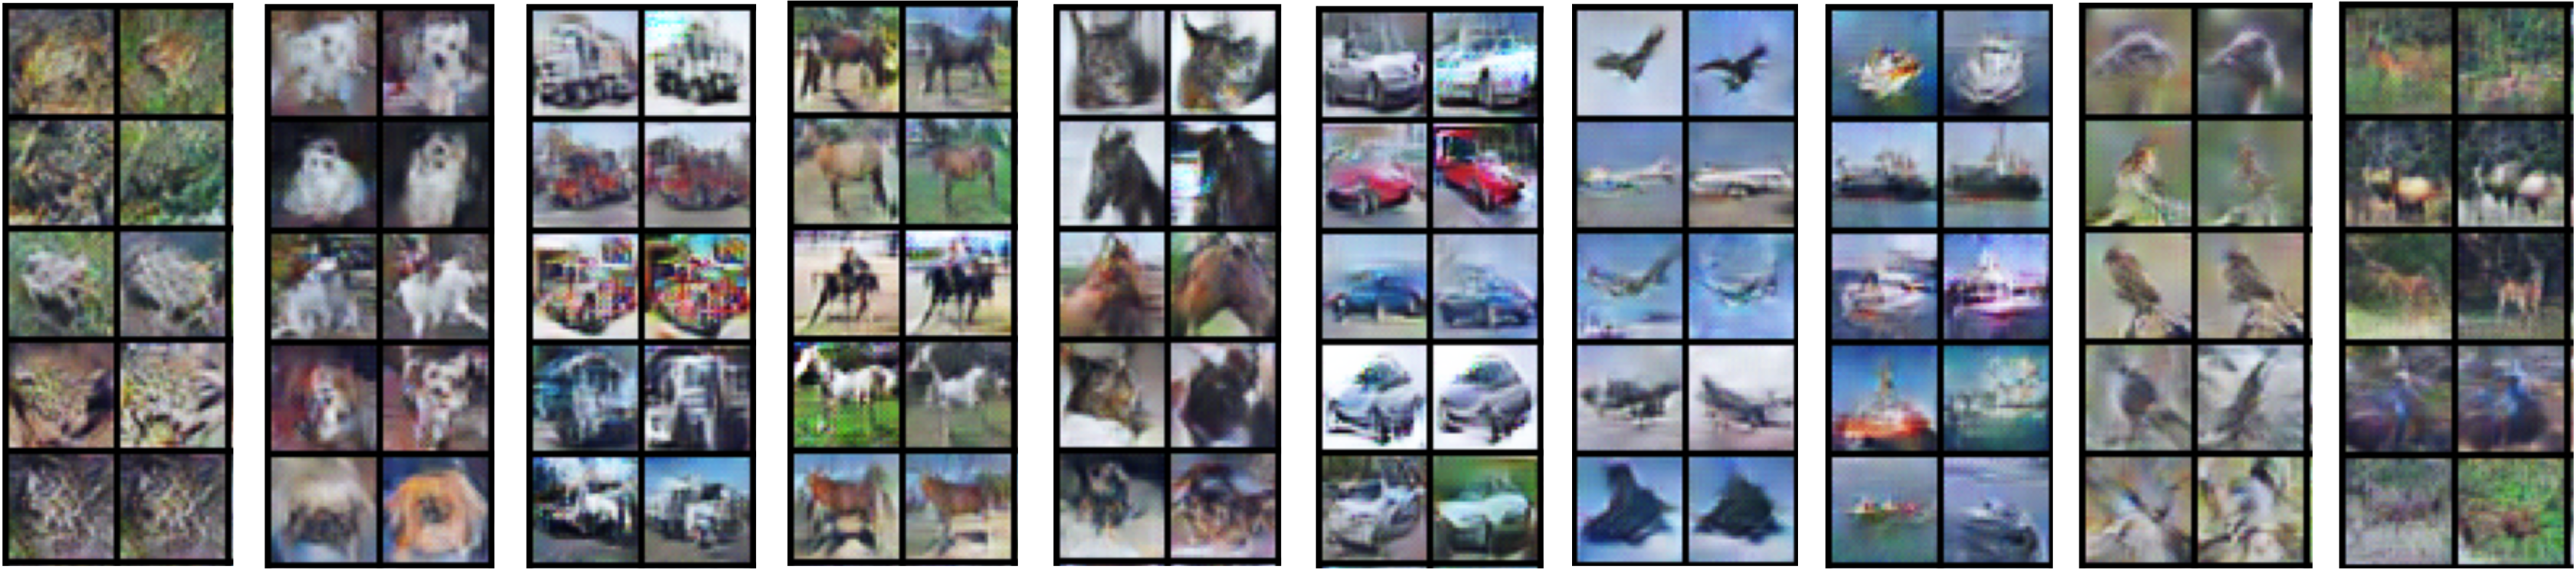
\includegraphics[width=0.95\textwidth]{figs_chap6/CIFAR10_generatedfromcluster.png}
    \caption{\small Unsupervised conditional image generation from each cluster of CIFAR-10, using u-CTRL. Images from different rows mean generation from different principal components of each cluster.}
    \label{fig:vis_clustering}
\end{figure}




% \section{Other Variations} 
% to be determined...

\section{Summary and Notes}
Materials presented in this chapter are based on a series of recent work on this topic: \cite{Dai-entropy-2022}, 
\cite{pai2022pursuit}, \cite{tong2023incremental}, and \cite{pmlr-v234-tong24a}.

In particular, Section \ref{sec:closed-loop-transcription} is based on the pioneering work of \cite{Dai-entropy-2022}. After that, the work of \cite{pai2022pursuit} has provided strong theoretical justifications for the closed-loop framework, at least for an ideal case. Section \ref{sec:class-wise-incremental} and Section \ref{sec:sample-wise-incremental} are based on the works of \cite{tong2023incremental} and \cite{pmlr-v234-tong24a}, respectively. They demonstrate that the closed-loop framework naturally supports incremental and continuous learning, either in a class-wise or sample-wise setting. The reader may refer to these papers for more technical and experimental details.

\section{Exercises and Extensions}

\end{document}